%!TEX TS-program = xelatex  
%!TEX encoding = UTF-8 Unicode  

\documentclass[12pt]{article}  
\usepackage{geometry}  
\geometry{letterpaper}  
\usepackage{fancyhdr}
\usepackage{extramarks}
\usepackage{amsmath}
\usepackage{amsthm}
\usepackage{amsfonts}
\usepackage{tikz}
\usepackage[plain]{algorithm}
\usepackage{algpseudocode} 
\usepackage{caption}
\usepackage{booktabs}
\usepackage{graphics}
\usepackage{amsmath}
\usepackage{amsfonts}

\usepackage{xltxtra,fontspec,xunicode}
\usepackage[slantfont,boldfont]{xeCJK}
\setCJKmainfont{宋体}   
\setmainfont{Optima}   
\defaultfontfeatures{Mapping=tex-text}  

\usepackage{xltxtra,fontspec,xunicode}
\usepackage[slantfont,boldfont]{xeCJK}
\setCJKmainfont{宋体}   
\setmainfont{Optima}   
\defaultfontfeatures{Mapping=tex-text}  

\XeTeXlinebreaklocale “zh”  
\XeTeXlinebreakskip = 0pt plus 1pt minus 0.1pt   
 
\usepackage{listings}
\usepackage{color}
\definecolor{dkgreen}{rgb}{0,0.6,0}
\definecolor{gray}{rgb}{0.5,0.5,0.5}
\definecolor{mauve}{rgb}{0.58,0,0.82}

\lstset{frame=tb,
  language=Java,
  aboveskip=3mm,
  belowskip=3mm,
  showstringspaces=false,
  columns=flexible,
  basicstyle={\small\ttfamily},
  numbers=none,
  numberstyle=\tiny\color{gray},
  keywordstyle=\color{blue},
  commentstyle=\color{dkgreen},
  stringstyle=\color{mauve},
  breaklines=true,
  breakatwhitespace=true,
  tabsize=3
} 

\topmargin=-0.45in
\evensidemargin=0in
\oddsidemargin=0in
\textwidth=6.5in
\textheight=9.0in
\headsep=0.25in

\linespread{1.1}

\pagestyle{fancy}
\lhead{\hmwkAuthorName}
\rhead{\hmwkClass}
\chead{\hmwkTitle}

\renewcommand\headrulewidth{0.4pt}
\renewcommand\footrulewidth{0.4pt}

\setlength\parindent{0pt}

% Homework Details

\newcommand{\hmwkTitle}{homework\ \#2}
\newcommand{\hmwkClass}{Deep Reinforcement Learning}
\newcommand{\hmwkAuthorName}{Tianxiao Hu}


\begin{document}
\pagebreak

\section{Problem 1}
(a)
\begin{equation}
\begin{aligned}
  & \nabla_\theta \mathbb{E}_{s_t, a_t \sim p(s_t, a_t)}[b_{(s_t)}]  \\
= & \nabla_\theta \mathbb{E}_{s_t, a_t}[\mathbb{E}_{a_t \sim \pi_\theta(a_t|s_t)}[b(s_t)]] \\
= & \mathbb{E} [\nabla_\theta \int \pi_\theta(a_t|s_t)b(s_t)da_t] \\
= & \mathbb{E}_{s_t \sim p(s_t)} [b(s_t) \cdot \int \nabla_\theta \pi_\theta(a_t|s_t)da_t] \\
= & \mathbb{E}_{s_t \sim p(s_t)}[b(s_t) \cdot \nabla_\theta \cdot \underbrace{\int \pi_\theta(a_t|s_t)da_t}_{\text{ = 1}}] \\
= & \mathbb{E}_{s_t \sim p(s_t)}[b(s_t) \cdot \nabla_\theta] \\
= & 0
\end{aligned}
\end{equation}

(b) \\
(1) Because this sequence is a markov decision process. Current state is only affected by last state. So conditioning on $(s_1, a_1, ..., a_{t^*-1}, s_{t^*})$ is equivalent to conditioning on $s_{t^*}$. \\
(2) 
\begin{equation}
\begin{aligned}
  & \nabla_\theta \mathbb{E}_{\tau \sim \pi_\theta(\tau)}[b(s_t^*)] \\
= & \nabla_\theta \cdot \int p(a_{t^*}|s_{t^*} \cdot s_{t^*-1} \cdot a_{t^*-1} \cdot \cdots \cdot s_1) p(s_{t^* \cdot s_{t^*-1} \cdot \cdots \cdot s_1}) b(s_{t^*}) da_{t^*}ds_{t^*}\cdot \cdots \cdot ds_1 \\
= & \nabla_\theta[\int p_\theta(a_{t^*}|s_{t^*}) \cdot p(s_{t^*}| ... ) b(s_{t^*})ds_{t^*}da_t] \underbrace{[\int p(s_{t^*-1} \cdot \cdots \cdot s_1)ds_{t^*-1} \cdot \cdots \cdot ds_1]}_{\text{= 1}} \\
= & \underbrace{\nabla_\theta \int p_\theta(a_{t^*}|s_{t^*})da_{t^*}}_{\text{=0}} \cdot \mathbb{E}_{s_{t^*} \sim p(s_{t^*})}[b(s_{t^*})]) \cdot 1 \\
= & 0
\end{aligned}
\end{equation}

\section{Problem 4}

\begin{figure}[!h]
\centering
\begin{minipage}[t]{0.48\textwidth}
\centering
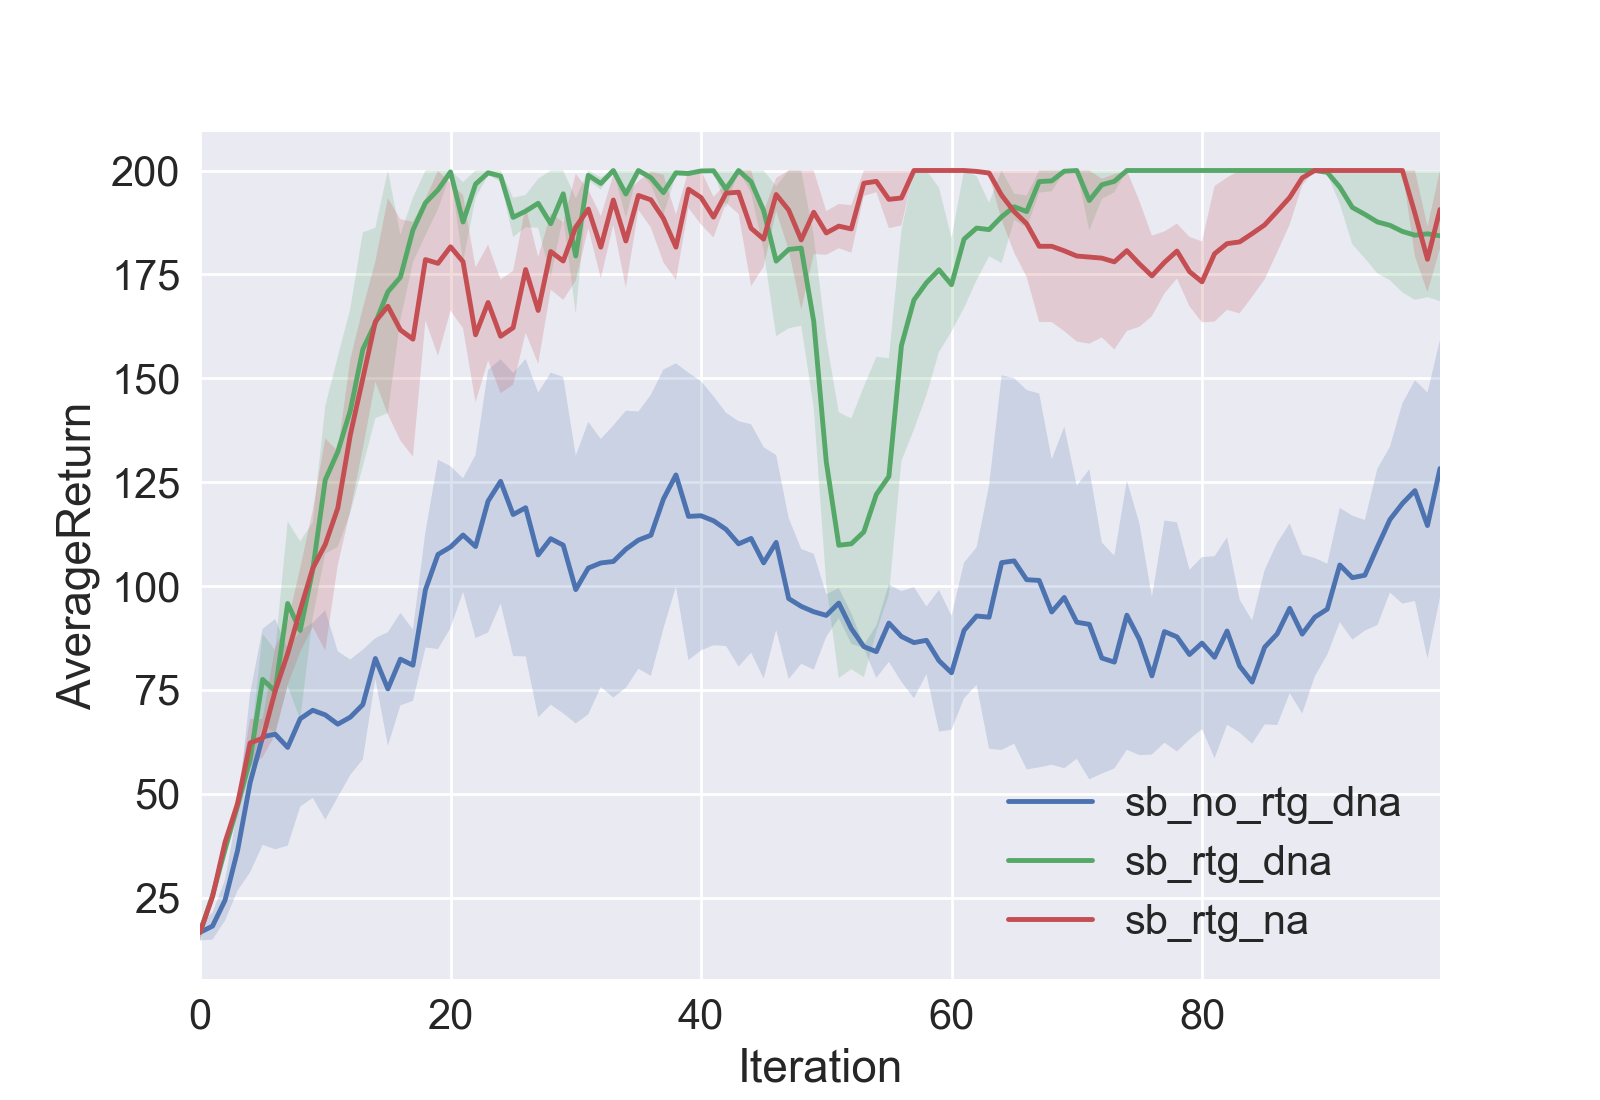
\includegraphics[width=8cm]{Figure_1.png}
\caption{Learning curves for small batch experiments.}
\end{minipage}
\begin{minipage}[t]{0.48\textwidth}
\centering
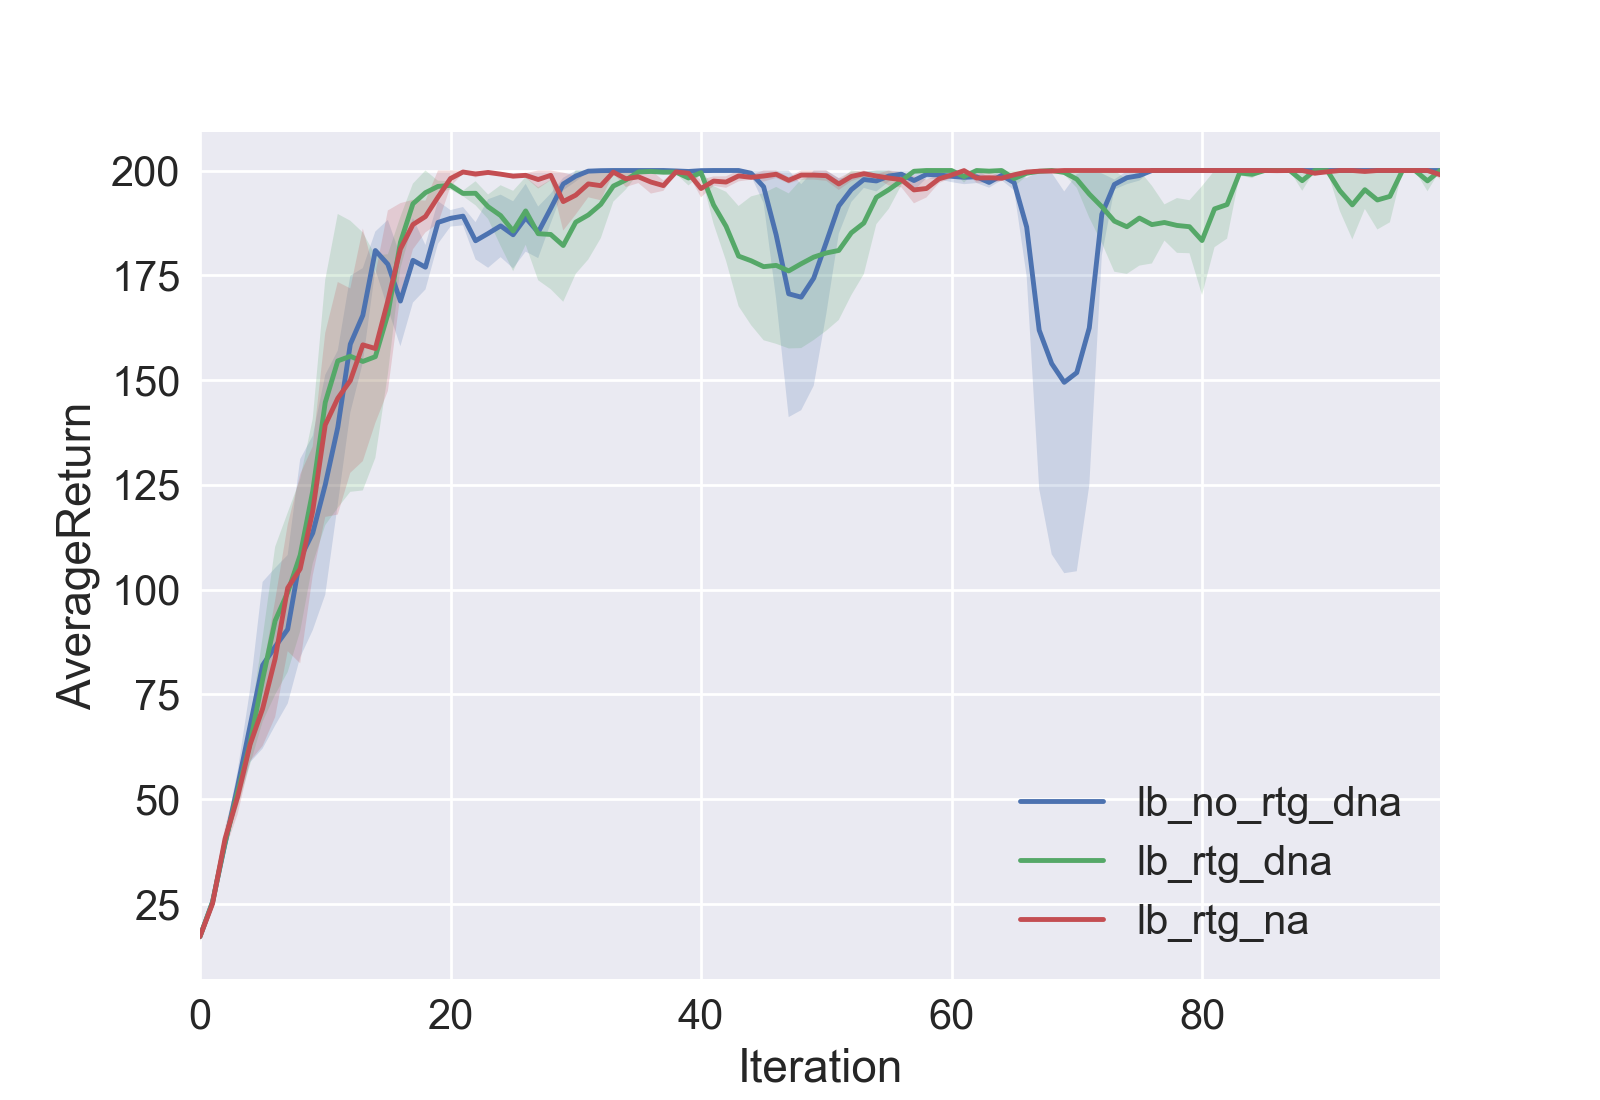
\includegraphics[width=8cm]{Figure_2.png}
\caption{Learning curves for large batch experiments.}
\end{minipage}
\end{figure}

\textbf{Answers:}\\
\begin{enumerate}
\item Which gradient estimator has better performance without advantage-centering, the trajectory-centric one, or the one using reward-to-go?\\
The one using reward-to-go have a better performance. From the learning curves for small batch experiments, we can see the green curve(reward-to-go) has a high average return than the blue curve(trajectory-centric).
\item Did advantage centering help?\\
It helps. From the learning curves for small batch experiments, we can see the red curve(with advantage-centering) fluctuates less than the green curve(without advantage-centering).
\item Did the batch size make an impact?\\
Yes, by comparing the learning curves between small batch experiments and large batch experiments, we find large batch experiments converge more quickly.
\end{enumerate}


\section{Problem 5}

\begin{figure}[!h]
\centering
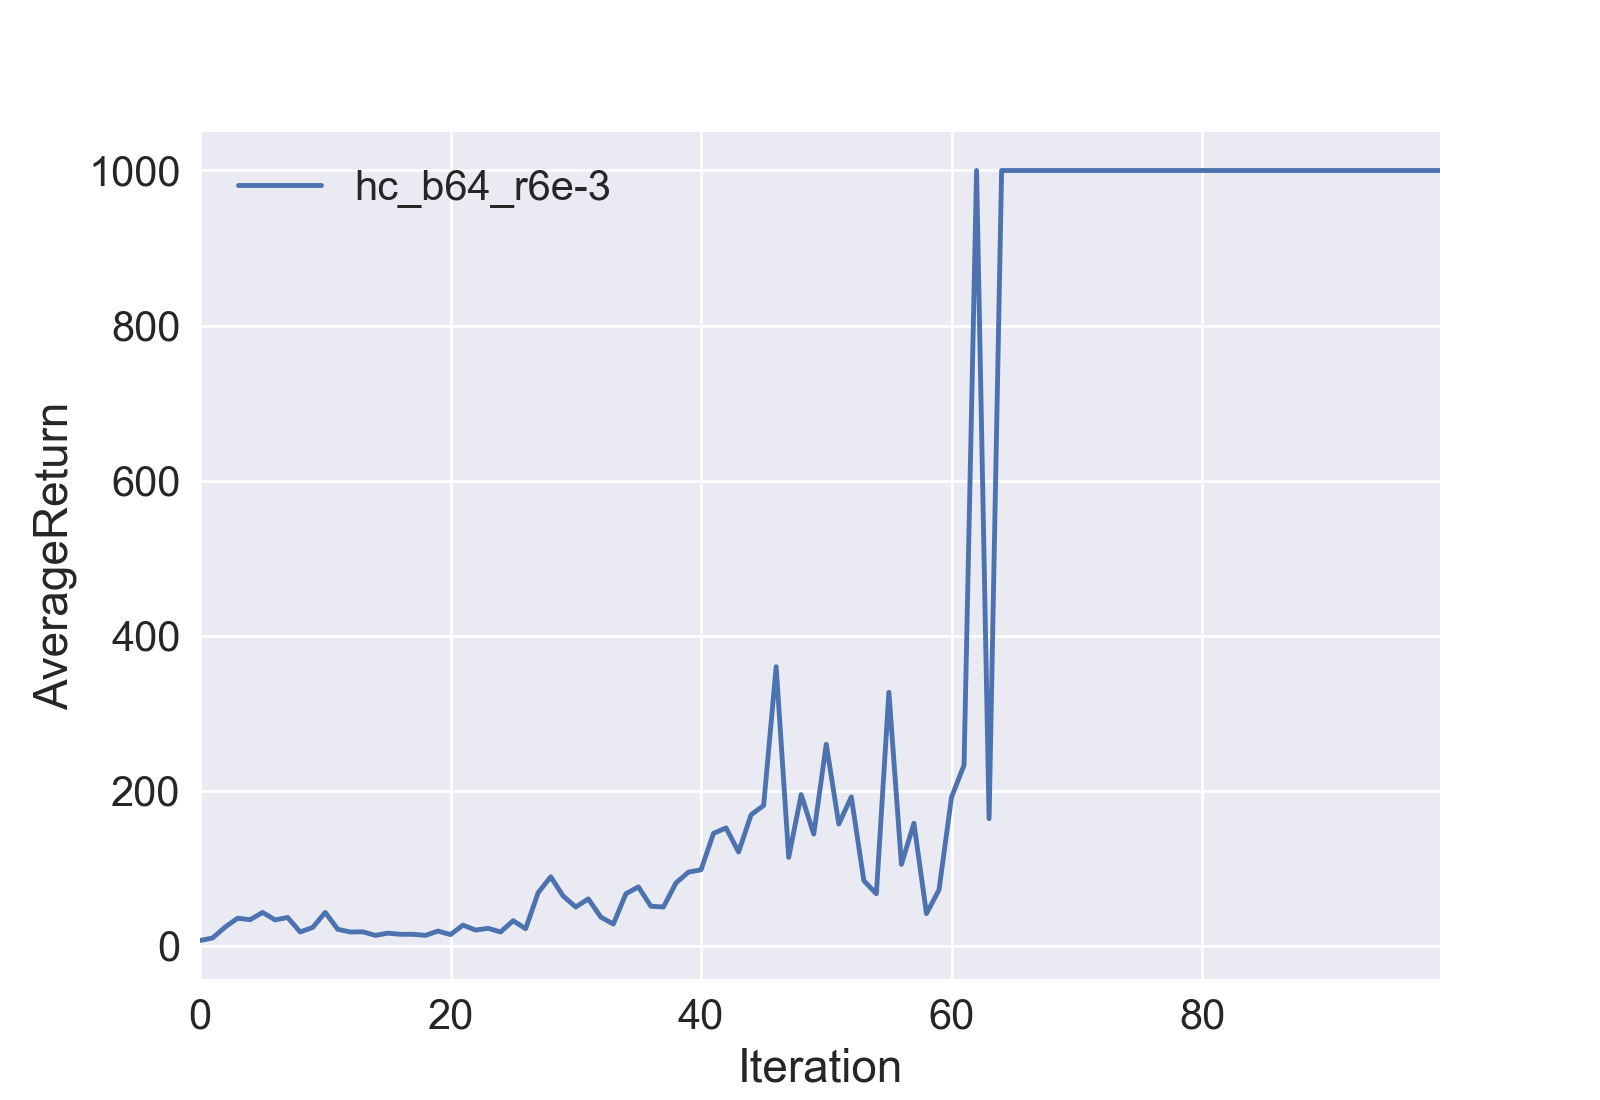
\includegraphics[width=3.8in]{Figure_3.png}
\caption{Learning curve with $b = 64$ and $lr = 0.006$. The policy gets to optimum at about iteration \#65.}
\end{figure}

\section{Problem 7}

\begin{figure}[!h]
\centering
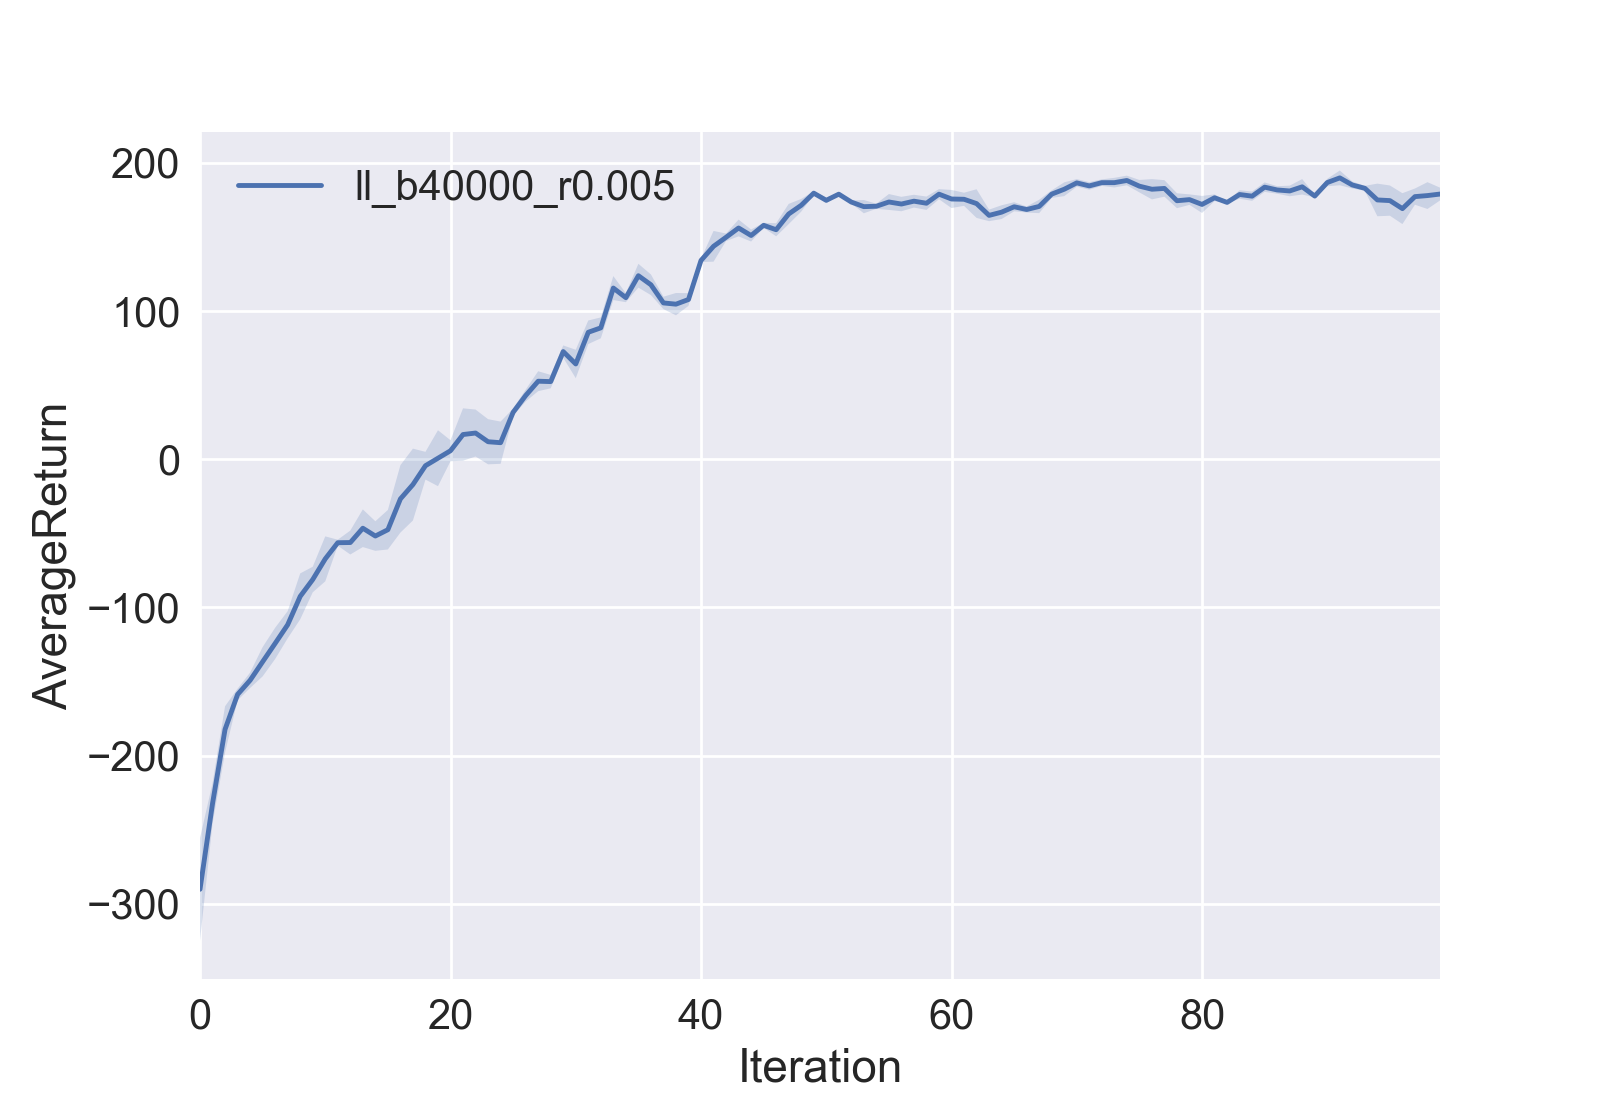
\includegraphics[width=3.8in]{Figure_4.png}
\caption{Learning curve for LunarLander. The policy finally achieved an average return of around 180.}
\end{figure}

\section{Problem 8}
After a $3 \times 3$ grid search, the best parameter set is $b = 50000, r = 0.02$.

\textbf{Answer:} How did the batch size and learning rate affect the performance? \\
Large batch size will help the learning curve use less iterations to converge. Using a small learning rate can make sure not to miss any local minimum, but adjust the learning rate larger properly can help the performance improve more quickly.

\begin{figure}[!h]
\centering
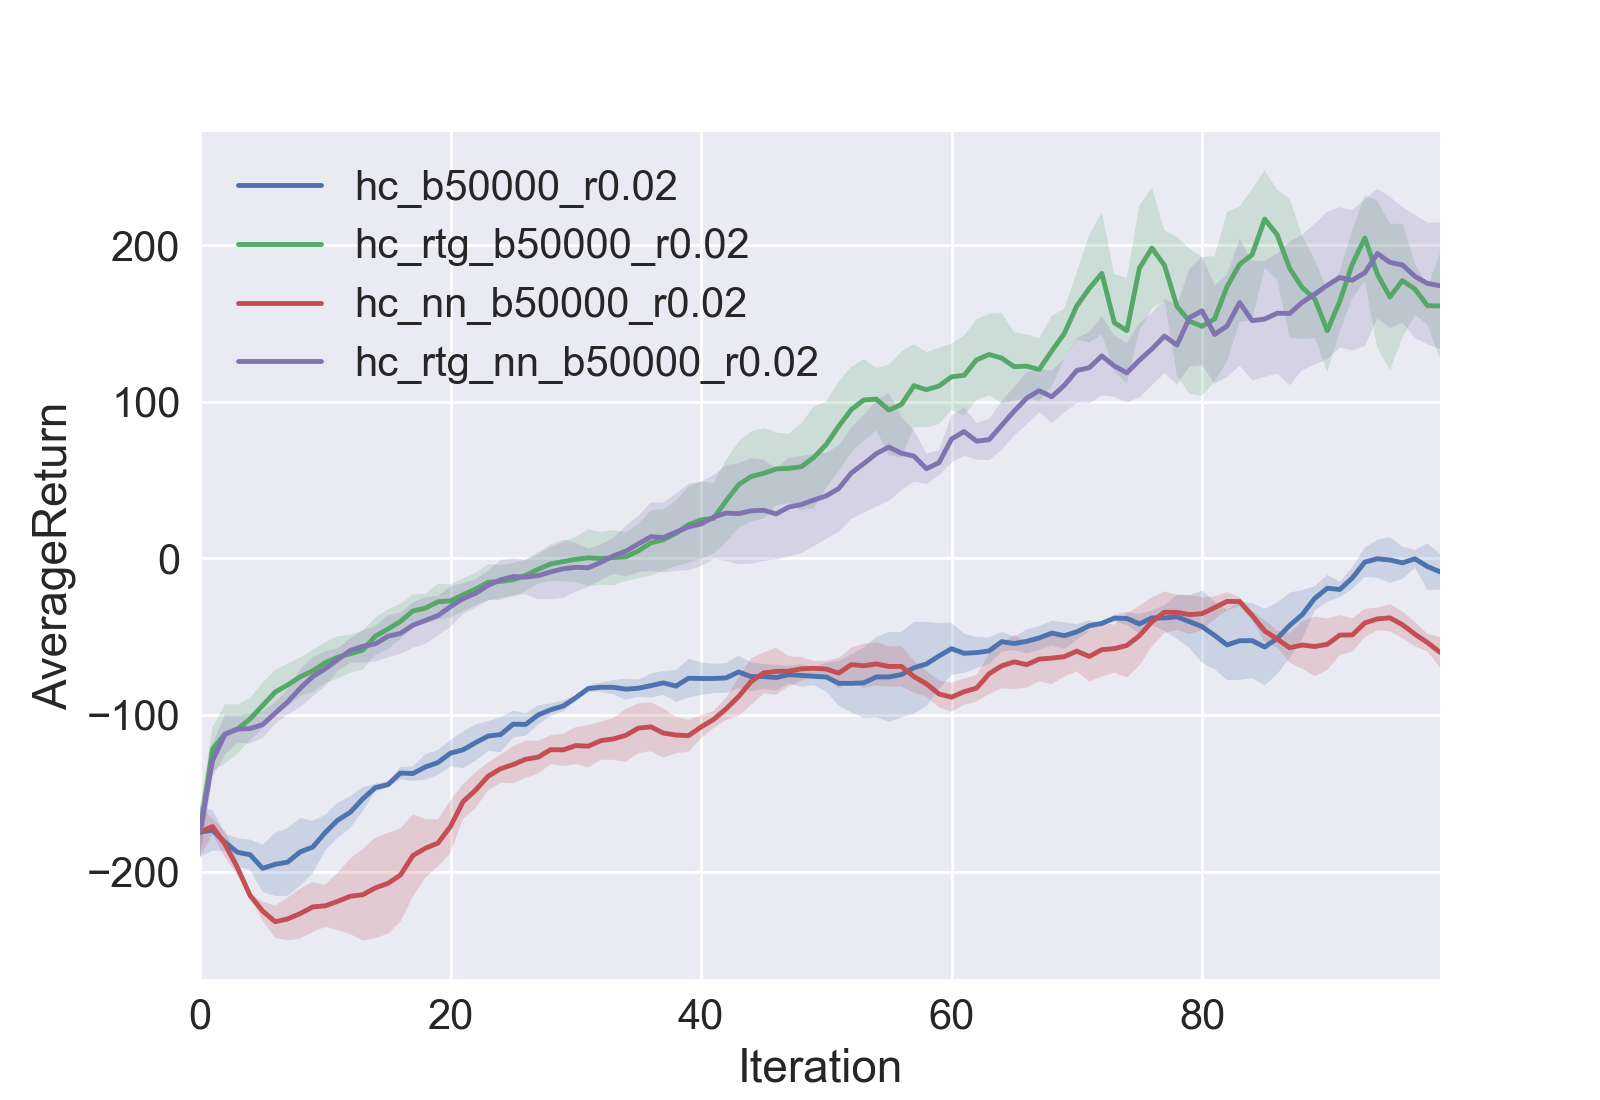
\includegraphics[width=3.7in]{Figure_5.png}
\caption{Learning curve for HalfCheetah with different parameters.}
\end{figure}

\end{document}  
  